\epigraph{\textit{'Smack my pitch up.'}}{The Prodigy (1997)}

\section{Optimal control of pitch/travel without feedback (10.2)}

%%%%%%%%%%%%%%%%%%%%%%%%%%%%%%%%%%%%%%%%%%%%%%%%%%%%%%%%%%%%
\subsection{State space form (10.2.1)}
%%%%%%%%%%%%%%%%%%%%%%%%%%%%%%%%%%%%%%%%%%%%%%%%%%%%%%%%%%%%
We want to write the model \eqref{eq:model1} in continuous time state space form with states and input as shown in \eqref{eq:state_and_input}.

\begin{equation}\label{eq:model1}
	\V{\dot{x}} = \M{A}_{c}\V{x} + \M{B}_{c}u
\end{equation}

\begin{equation}\label{eq:state_and_input}
\begin{aligned}
	\V{x} 	&= \begin{bmatrix}\lambda & r & p & \dot{p} \end{bmatrix}\transpose \\
	u 		&= p_{c}
\end{aligned}
\end{equation}
The equations of motion for the states are shown in \eqref{eq:state_equations} and the constants used are defined in \eqref{eq:K1K2}. These are derived in detail in \cite{_helicopter_2015}, and will be used without any further explanation here. This also applies for \eqref{eq:state_eqns} in section \ref{10.4.1}. 

\begin{equation}\label{eq:state_equations}
\begin{aligned}
	\dot{\lambda} 	&= r \\
	\dot{r} 		&= - K_{a} p \\
	\dot{p} 		&= \dot{p} \\
	\ddot{p} 		&= K_{1} K_{pp} (p_{c} - p) - K_{1} K_{pd} \dot{p}
\end{aligned}
\end{equation}

\begin{equation}\label{eq:K1K2}
\begin{aligned}
	K_{1} &= \frac{K_{f} l_{n}}{J_{p}} \\
	K_{2} &= \frac{K_{p} l_{a}}{J_{t}}
\end{aligned}
\end{equation}
The above gives the result in \eqref{eq:state_space_matrices}.

\begin{equation}\label{eq:state_space_matrices}
	\V{\dot{x}} =
	\underbrace{
		\begin{bmatrix}
			0 & 1 & 0 				& 0 \\
			0 & 0 & -K_{2} 			& 0 \\
			0 & 0 & 0 				& 1 \\
			0 & 0 & -K_{1}K_{pp}	& -K_{1}K_{pd}
		\end{bmatrix}
	}_{\M{A}_{c}}
	\V{x} +
	\underbrace{
		\begin{bmatrix}
			0 \\ 0 \\ 0 \\ K_{1}K_{pp}
		\end{bmatrix}
	}_{\M{B}_{c}}
	u
\end{equation}


%%%%%%%%%%%%%%%%%%%%%%%%%%%%%%%%%%%%%%%%%%%%%%%%%%%%%%%%%%%%
\subsection{Model discussion (10.2.1)}
%%%%%%%%%%%%%%%%%%%%%%%%%%%%%%%%%%%%%%%%%%%%%%%%%%%%%%%%%%%%
The states are travel, travel rate, pitch, and pitch rate. The controller output is the pitch setpoint to be used by the already implemented controller which in turn calculates voltage inputs for the plant. Thus, we are modelling not the helicopter alone, but a system that consists of the helicopter along with the given controller. This corresponds with figure 7 in the exercise text \cite{_helicopter_2015}.


%%%%%%%%%%%%%%%%%%%%%%%%%%%%%%%%%%%%%%%%%%%%%%%%%%%%%%%%%%%%
\subsection{Discretization (10.2.2)}\label{sec:disc1}
%%%%%%%%%%%%%%%%%%%%%%%%%%%%%%%%%%%%%%%%%%%%%%%%%%%%%%%%%%%%
We discretize the system by the Forward Euler Method. The general definition of the method and how it relates to our system is described by equations \eqref{eq:forward_euler} and \eqref{eq:euler_func}, respectively.

\begin{equation}\label{eq:forward_euler}
	y_{k+1} = y_{k} + h f(x_{k}, y_{k})
\end{equation}

\begin{equation}\label{eq:euler_func}
	f = \left( \M{A}_{c} \V{x}_{k} + \M{B}_c u_{k} \right)
\end{equation}
Using \eqref{eq:forward_euler} and \eqref{eq:euler_func}, we can find the matrices of the discretized system, as shown in \eqref{eq:disc}, \eqref{eq:disc_matrix_A}, and \eqref{eq:disc_matrix_B}.

\begin{equation}\label{eq:disc}
\begin{aligned}
	\V{x}_{k+1} &= \V{x}_{k} + \left( \M{A}_{c} \V{x}_{k} + \M{B}_c u_{k} \right) h \\
				&= \V{x}_{k} + h\M{A}_{c}\V{x}_{k} + h\M{B}_{c}u_{k} \\
				&= \left( \Mc{I} + h\M{A}_{c} \right) \V{x}_{k} + h\M{B}_{c}u_{k} \\
				&= \M{A}\V{x}_{k} + \M{B}u_{k}
\end{aligned}
\end{equation}

\begin{equation}\label{eq:disc_matrix_A}
	\M{A} = \Mc{I} + h\M{A}_{c} =
	\begin{bmatrix}
		1 & h & 0 & 0 \\
		0 & 1 & -K_{2}h & 0 \\
		0 & 0 & 1 & h \\
		0 & 0 & -K_{1}K_{pp}h	& 1-K_{1}K_{pd}h
	\end{bmatrix}
\end{equation}

\begin{equation}\label{eq:disc_matrix_B}
	\M{B} = h\M{B}_c =
	\begin{bmatrix} 0 \\ 0 \\ 0 \\ K_{1}K_{pp}h \end{bmatrix}
\end{equation}


%%%%%%%%%%%%%%%%%%%%%%%%%%%%%%%%%%%%%%%%%%%%%%%%%%%%%%%%%%%%
\subsection{Discussion of the cost function (10.2.3)}
%%%%%%%%%%%%%%%%%%%%%%%%%%%%%%%%%%%%%%%%%%%%%%%%%%%%%%%%%%%%
We are given the cost function \eqref{eq:cost_function} from the exercise text \cite{_helicopter_2015} that we want to minimize, with the constraints given by \eqref{eq:cost_constraint}.


\begin{equation} \label {eq:cost_function}
	\phi = \sum\limits_{i=1}^N (\lambda_i - \lambda_f)^2 + q p_{ci}^2, \quad q \geq 0 
\end{equation}

\begin{equation} \label{eq:cost_constraint}
	|p_k| \leq \frac{30 \pi}{180}, \quad k \in \{ 1, ..., N \}
\end{equation}

This cost function focuses on the error between $\lambda_i$ and $\lambda_f$.
It is a  quadratic least-square function and we will therefore use quadratic programming to make the error of $\lambda_i$ and $\lambda_f$ as small as possible.  
The second part of the cost function consists of the pitch reference input, and a constant $q$ which decides how much you should focus on it. This part can lead to unwanted effects, which are discussed in \ref{unwanted}.

\textbf{TODO we must lay in some plots}

%%%%%%%%%%%%%%%%%%%%%%%%%%%%%%%%%%%%%%%%%%%%%%%%%%%%%%%%%%%%
\subsection{Procedure for solving the optimization problem (10.2.3)} \label{optimalProcedure}
%%%%%%%%%%%%%%%%%%%%%%%%%%%%%%%%%%%%%%%%%%%%%%%%%%%%%%%%%%%%

The objective is to calculate an optimal trajectory for moving the helicopter from $x_0 = \begin{bmatrix} \lambda_0 & 0 & 0 & 0 \end{bmatrix} \transpose$ to $x_f = \begin{bmatrix} \lambda_f & 0 & 0 & 0 \end{bmatrix} \transpose$ with constant elevation angle. In this case we use $\lambda_0 = \pi$ and $\lambda_f = 0$.

We start by declaring the constants given in Table \ref{table:constants}, the $\M{A}$ and $\M{B}$ matrices given in \eqref{eq:state_space_matrices}, and $x_0$ given above. Then we implements the constraints in \eqref{eq:cost_constraint} using the following code:

\begin{lstlisting}

% Bounds

ul 	    = -30*pi/180;        % Lower bound on control -- u1
uu 	    = 30*pi/180;         % Upper bound on control -- u1

xl      = -Inf*ones(mx,1);   % Lower bound on states (no bound)
xu      = Inf*ones(mx,1);    % Upper bound on states (no bound)
xl(3)   = ul;                % Lower bound on state x3
xu(3)   = uu;                % Upper bound on state x3

% Generate constraints on measurements and inputs

[vlb,vub]       = genBegr2(N,M,xl,xu,ul,uu);
vlb(N*mx+M*mu)  = 0;         % We want the last input to be zero
vub(N*mx+M*mu)  = 0;         % We want the last input to be zero

\end{lstlisting}
where \texttt{genBegr2} is like this:

%NB denne koden er hentet fra nettet, skriv kilde
\newline
\begin{lstlisting} %få kommentarene på en linje, ser mye bedre ut

function [vlb,vub] = genBegr2(N,M,xl,xu,ul,uu);

vlb_x	= repmat(xl,N,1);	% Lager begrensning for hvert tidsskritt
vub_x	= repmat(xu,N,1);	% Lager begrensning for hvert tidsskritt

vlb_u	= repmat(ul,M,1);	% Lager begrensning for hvert tidsskritt
vub_u	= repmat(uu,M,1);	% Lager begrensning for hvert tidsskritt

vlb	    = [vlb_x; vlb_u];	% Setter sammen begrensningene for xl og ul
vub	    = [vub_x; vub_u];	% Setter sammen begrensningene for xu og uu
\end{lstlisting}

After that we find weight matrices for the QP problem and the matrices for the equality constrains:
\begin{lstlisting}
% Generate the matrix Q and the vector c (objecitve function weights in the QP problem) 

Q1 = zeros(mx,mx);
Q1(1,1) = 1;                	% Weight on state x1
Q1(2,2) = 0;                	% Weight on state x2
Q1(3,3) = 0;                	% Weight on state x3
Q1(4,4) = 0;                	% Weight on state x4
P1 = q;                     	% Weight on input
Q = 2*genq2(Q1,P1,N,M,mu);  	% Generate Q
c = zeros(N*mx+M*mu,1);     	% Generate c

% Generate system matrixes for linear model

Aeq = gena2(A1,B1,N,mx,mu); 	% Generate A
beq = zeros(1, size(Aeq,1));	% Generate b
beq(1:mx) = A1*x0; 	        	% Initial value
\end{lstlisting}
using \texttt{genq2} 

\begin{lstlisting} %NB denne koden er hentet fra nettet, skriv kilde

function Q = genq2(Q1,P1,N,M,mu)

p1	= blkdiag2(P1,M);
q1	= blkdiag2(Q1,N);

Q	= blkdiag(q1,p1); 
\end{lstlisting}
and \texttt{gena2}

\begin{lstlisting} %NB denne koden er hentet fra nettet, skriv kilde

function A = gena2(A1,B1,N,mx,mu)

A 	= zeros(N*mx,N*mx+N*mu);
b1	= blkdiag2(-B1,N);
a1	= eye(N*mx);
for i=1:(N-1)
  a1([(i*mx+1):((i+1)*mx)],[((i-1)*mx+1):(i*mx)])=-A1;
end
A	= [a1 b1];
\end{lstlisting}

At last we can solve the quadratic problem using \texttt{quadprog}:

\begin{lstlisting}
	[z,lambda] = quadprog(Q, c, [], [], Aeq, beq, vlb, vub, z0);
\end{lstlisting}
where $\M{Z} = \begin{bmatrix} \V{x}_1 & \V{x}_2 & ... & \V{x}_N & u_1 & u_2 & ... & u_N \end{bmatrix} \transpose$. The complete code is listed in the appendix (ref her!). We find the desired states and get these plots, using three different value of q:

\textbf{TODO: plots here} 

%%%%%%%%%%%%%%%%%%%%%%%%%%%%%%%%%%%%%%%%%%%%%%%%%%%%%%%%%%%%
\subsection{Discussion of unwanted effects (10.2.3)\label{unwanted}}
%%%%%%%%%%%%%%%%%%%%%%%%%%%%%%%%%%%%%%%%%%%%%%%%%%%%%%%%%%%%
When $\lambda = \lambda_f$, the first part of the cost function will be 0, and the QP algorithm will try to minimize the pitch. This will set the pitch to 0, which could make the helicopter overshoot and not stop at the reference. This can lead to the helicopter oscillating around this point.


%%%%%%%%%%%%%%%%%%%%%%%%%%%%%%%%%%%%%%%%%%%%%%%%%%%%%%%%%%%%
\subsection{Deviation and desired behaviour of helicopter (10.2.4)}
%%%%%%%%%%%%%%%%%%%%%%%%%%%%%%%%%%%%%%%%%%%%%%%%%%%%%%%%%%%%
Now we want to use the optimal input found in \ref{optimalProcedure} as an input to our physical helicopter system. We do this using Simulink with QuaRC. It will look like this:

\begin{figure}[H]
	\centering
	\includegraphics[width=\textwidth, trim=2cm 6cm 2cm 2cm]{simulinkmodels/heldag2}
	\caption{Simulink model of the system}
	\label{fig:heldag2}
\end{figure}

The helicopter does not stop in the desired end point, as the QP algorithm overcompensates for the time needed to brake, and the helicopter starts gliding back in the opposite direction. This is shown in the plots.

\begin{figure}[H]
	\centering
	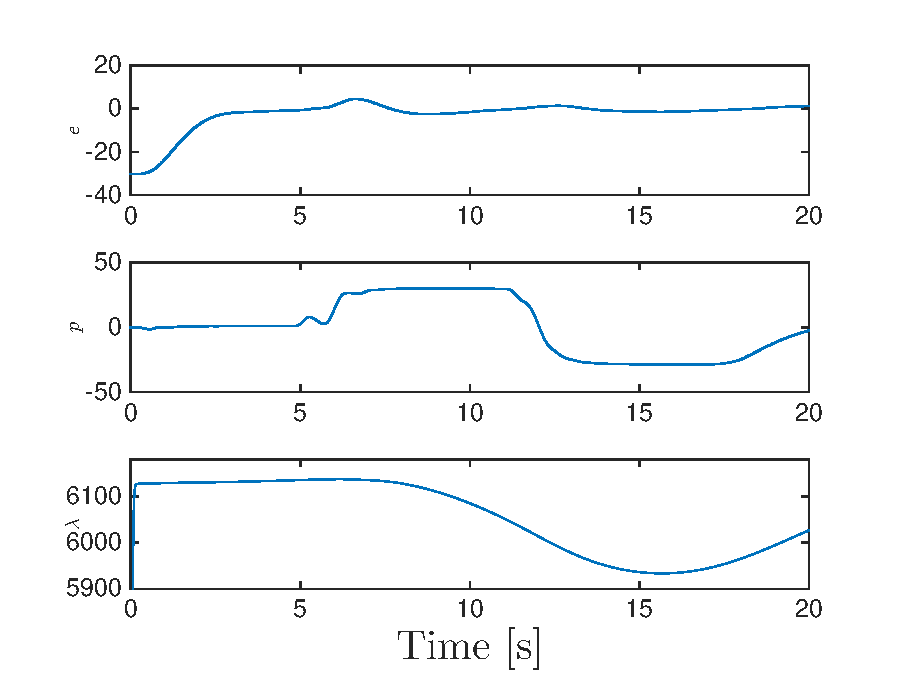
\includegraphics[width=\textwidth]{day2}
	\caption{Actual values day 2}
	\label{fig:day2}
\end{figure}
